\chapter{The Comparative Study}
\label{chap:Comparative_Study}

This chapter presents the comparative study.


The eye blink countermeasure used in this thesis uses a similar technique applied in Motion Correlation countermeasure\cite{AnjosIJCB2011} as discussed in the Section \ref{sec:scene_cues}. In this countermeasure 

The difference BLA BLA.
Figure \ref{fig:eye_blink} shows the eye blink detection scheme used in the countermeasure.

\begin{figure}[!btb]
\begin{center}
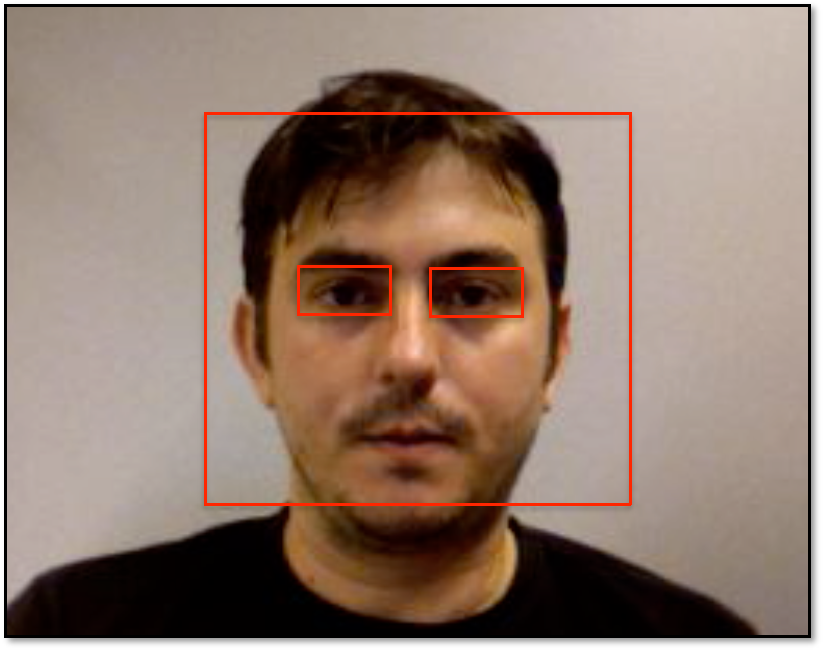
\includegraphics [width=10cm] {images/eye_blink.pdf}
\caption[Eye blink countermeasure scheme]{Eye blink countermeasure scheme}
\label{fig:eye_blink}
\end{center}
\end{figure}


\section{Evaluation Protocol}
\label{sec:Evaluation_Protocol}

Firstly, we study how the countermeasures, presented in Section \ref{sec:countermeasures}, will perform in a more realistic condition. This condition consists in training and tuning each one of the countermeasures with one face anti-spoofing database and testing with another one. To report the performance in such a scenario, two evaluation protocols were designed to work with the databases described in Section \ref{sec_replay}. These protocols are the "intra-test" protocol and the "inter-test" protocol.


\subsection{Intra-test Protocol}

The intra-test protocol is equivalent to the database normal protocol. It consists in training, tuning and testing a countermeasure with the respectively training set, development set and test set of such a database. With this protocol, it is possible to evaluate the performance and the generalization power of a countermeasure within one database. 

\subsection{Inter-test Protocol}

The inter-test protocol evaluates the countermeasure performance in a more realistic scenario, close to real usage conditions. It consists in training and tuning a countermeasure with the training set and development set of one database and test it with the test set of another one. With this protocol, it is possible to evaluate the performance and the generalization power of a countermeasure in a set of unseen types of attacks.


\subsection{Evaluation Metrics}

The Replay Attack Database provides a protocol for objective evaluation of a given countermeasure. To mitigate overfitting, such a protocol defines three non-overlapping partitions: the training, development and test set. The training set should be used to train the countermeasure, the development set is used to tune the countermeasure. The test set must be used only to report results. 

The CASIA FASD lacks a specific development set; this database has only a train and a test set. To mitigate the over-fitting in this database, the train set was split into five partitions and a 5-fold cross-validation training was done. For that, 4 folds were used for training and 1 fold was used to tune the countermeasure. With this strategy, both databases have a train set, a development set (to tune the countermeasure) and a test set, so it is possible to merge them.

The performance of each countermeasure, using the test set of each database, is reported with the Half Total Error Rate ($HTER$): 

\begin{equation}
\label{eq:HTER}
HTER(D_2)=\frac{FAR(\tau(D_1),D_2)+ FRR(\tau(D_1),D_2)} {2} ,
\end{equation}
where $\tau(D_n)$ is a threshold, $D_n$ is the dataset, $FAR$ is the False Acceptance Rate in the database $D_2$ and $FRR$ is the False Rejection Rate in the database $D_2$. In this protocol, the value of $\tau(D_n)$ is estimated on the Equal Error Rate (EER) using the development set of the database $D_1$. In this Equation when $D_1 = D_2$, we have the intra-test protocol and when $D_1 \neq D_2$, we have the inter-test protocol.

Because of 5-fold cross validation protocol, for the CASIA FASD 5 results were generated. The average of $HTER$ was provided as a final result.

In order to eliminate the face detector influence, the same face detector, based on Modified Census Transform (MCT) features \cite{froba2004face}, was used for both databases.

ROC CURVES

\section{Evaluated countermeasures}
\label{sec:Evaluated_countermeasures}

For this comparative study were selected four countermeasures very representative according to the state of the art in this research. Next subsections will describe each one and the hyper-parameters set BLA BLA BLA.

It is important to remark that each countermeasure TYPE OF CUES  

In this work we follow the tuning suggested by the authors.

\subsection{Motion Correlation}

As presented in Section \ref{sec:scene_cues}, the Motion correlation \cite{AnjosIJCB2011} countermeasure measures the correlation between the face and it background. With some contributions by our side, the source code of this countermeasure is freely available \footnote{https://github.com/bioidiap/antispoofing.motion/}. There are, basically, two hyper-parameters in this countermeasure. The first one is the number of frames used to compute the 5 quantities. The second one is the binary classifier.

As the authors suggested, twenty frames to compute the 5 quantities are sufficient to the algorithm converge in their experiments. The classifier suggested in the paper was one based on Multi-layer Perceptron. This classifier has, basically, the number of hidden layers and the number neurons in each hidden layer. As the good tradeoff between computational complexity and performance, the authors suggested one hidden layer and five neurons in this hidden layer.

\subsection{Textures with $LBP$}

Presented in Section \ref{sec:quality_assessment}, the countermeasure based on Textures with $LBP$ \cite{ChingovskaBIOSIG2012} and \cite{maatta2011face} explore the differences in texture properties between real accesses and attacks in single frames. 

There are, basically, three hyper-parameters in this countermeasure. The first one is the geometrically normalized face size. The authors suggested a face size of $64 \times 64$ pixels. The second one is the configuration of the $LBP$ texture descriptor. The $LBP$ itself has several hyper-parameters \ref{inen2011computer} and the authors of both papers stressed only some of that. In this thesis we will follow the setup suggested by \cite{ChingovskaBIOSIG2012} using the $LBP_{8,1}^{u2}$. Finally the last hyper-parameter is the binary classifier. The best classifier tested by \cite{ChingovskaBIOSIG2012} was the Support Vector Machines (SVM) using the Radial Basis Function (RBF). For this classifier the parameter $C$ (the cost of the loss function) and the $\gamma$ parameter (the variance of the radial function) was set to $1$ and $0.1$ respectivelly.

\subsection{Dynamic Textures with $LBP-TOP$}

Presented in the Chapter \ref{chap:Proposed_Countermeasures}, the countermeasure based on dynamic textures with $LBP-TOP$, explore the texture dynamics to detect attacks in a frame sequence.









